% !TeX program = xelatex
% ICEC30/ICMC2026 poster, SMU/Gemini two-column IMRD&C layout.
% Keep Overleaf builds self-contained: local builds set TEXINPUTS in build.ps1,
% while Overleaf needs the bundled support folders declared from the source.
\makeatletter
\def\input@path{{./}{vendor/beamerposter/}{vendor/gemini-local/}{vendor/beamerposter/translator_pkg/translator/}}
\makeatother

\documentclass[final]{beamer}

\usepackage[size=custom,width=90,height=150,scale=1.13]{beamerposter}
\usetheme{gemini}
\usecolortheme{smu}
\useinnertheme{rectangles}
\usepackage{graphicx}
\usepackage{booktabs}
\usepackage{array}
\usepackage{amsmath}
\usepackage{tikz}
\usetikzlibrary{arrows.meta,positioning}

\IfFontExistsTF{Times New Roman}{%
  \setmainfont{Times New Roman}[Ligatures=TeX]
  \setsansfont{Times New Roman}[Ligatures=TeX]
}{%
  \setmainfont{TeX Gyre Termes}[Ligatures=TeX]
  \setsansfont{TeX Gyre Termes}[Ligatures=TeX]
}
\IfFontExistsTF{Courier New}{%
  \setmonofont{Courier New}[Scale=MatchLowercase]
}{%
  \setmonofont{TeX Gyre Cursor}[Scale=MatchLowercase]
}
\renewcommand{\familydefault}{\rmdefault}

\setbeamerfont{headline}{family=\rmfamily}
\setbeamerfont{headline title}{family=\rmfamily,size=\fontsize{31}{36}\selectfont,series=\bfseries}
\setbeamerfont{headline author}{family=\rmfamily,size=\fontsize{15.5}{18.5}\selectfont}
\setbeamerfont{headline institute}{family=\rmfamily,size=\fontsize{13.5}{16}\selectfont}
\setbeamerfont{block title}{family=\rmfamily,size=\fontsize{20.2}{23.6}\selectfont,series=\bfseries}
\setbeamerfont{block body}{family=\rmfamily,size=\fontsize{14.8}{17.5}\selectfont}
\setbeamerfont{heading}{family=\rmfamily,series=\bfseries}
\setbeamerfont{caption}{family=\rmfamily,size=\fontsize{9.8}{11.4}\selectfont}
\setbeamerfont{footline}{family=\rmfamily}
\setlength{\abovecaptionskip}{0.4ex}
\setlength{\belowcaptionskip}{0.2ex}

\newlength{\sepwidth}
\newlength{\colwidth}
\setlength{\sepwidth}{0.020\paperwidth}
\setlength{\colwidth}{0.470\paperwidth}
\newcommand{\separatorcolumn}{\begin{column}{\sepwidth}\end{column}}

\newcommand{\tightlist}{\setlength{\itemsep}{0.08ex}\setlength{\topsep}{0.08ex}\setlength{\parsep}{0pt}\setlength{\parskip}{0pt}}
\newcommand{\compacttable}{\fontsize{10.4}{12.2}\selectfont\setlength{\tabcolsep}{0.35em}}
\newcommand{\smallnote}[1]{{\fontsize{9.4}{11.0}\selectfont\color{black!64}#1}\par}
\newcommand{\metric}[2]{%
  \begin{minipage}[t]{0.235\linewidth}
    \centering
    {\usebeamercolor[fg]{structure}\bfseries\fontsize{25}{28}\selectfont #1}\par
    {\fontsize{9.2}{10.8}\selectfont #2}
  \end{minipage}}
\newenvironment{posterblock}[5]{%
  \begingroup
  \setbeamercolor{block title}{fg=#1,bg=#2}%
  \setbeamercolor{block separator}{bg=#3}%
  \setbeamercolor{block body}{fg=smuink,bg=#4}%
  \begin{block}{#5}%
}{%
  \end{block}%
  \endgroup
}

\title{Experimental Validation of a Corrugated Membrane for Large-Scale Liquid Hydrogen Cargo Containment}
\author{Qian Wang \and Xinyuan Liu \and Anran Li \and Honghai Tian}
\institute[ZIAC]{Zhongshan Institute of Advanced Cryogenic Technology, China}

\logoleft{
\includegraphics[height=5.6cm]{assets/institute_logo.png}}
\logoright{\begingroup\setlength{\fboxsep}{0.22cm}\colorbox{white}{
\includegraphics[height=4.5cm]{assets/conference_logo.png}}\endgroup}

\footercontent{
  P1-061 | Poster Session I | Exhibition Hall (111+112) | June 23, 2026 | 14:00--16:00
  \hfill
  Poster size: 0.9 m (W) x 1.5 m (H)
  \hfill
  \texttt{wangqian@ziac.cn}; \texttt{liuxinyuan@ziac.cn}
}

\begin{document}
\begin{frame}[t]

\begin{columns}[t]
\separatorcolumn

\begin{column}{\colwidth}

\begin{posterblock}{white}{smunavy}{smublue}{smulight}{Introduction}
Large-scale LH$_2$ cargo containment needs a metallic primary barrier that is leak-tight, formable, and tolerant of the in-plane displacement generated when the tank system cools from ambient temperature to cryogenic service. If this displacement is carried mainly by membrane stretching, local strain concentration can become a direct risk for cracking, leakage, and loss of containment reliability.

A corrugated 316L membrane is introduced to turn this constraint into a geometric compliance problem. The selected cross-corrugated profile is expected to accommodate imposed displacement through local bending and rotation of crests, valleys, and side-wall transitions, thereby lowering the uniform stretching demand on the thin sheet.

The remaining question is experimental rather than purely geometric: after patent-based forming, specimen preparation, and cyclic loading, does the membrane still follow the intended strain-release mechanism, and can an assembled module retain preliminary integrity after cryogenic cycling?

This poster therefore links three checks into one validation chain: DIC/PLC maps where imposed displacement is released, AE monitors cyclic damage activity during repeated loading, and pressure-hold plus helium leak testing are used as the pressure-retention method to verify assembly integrity after LN$_2$ fill/drain cycles.

\begin{center}
\resizebox{0.96\linewidth}{!}{%
\begin{tikzpicture}[
  font=\rmfamily,
  panel/.style={rounded corners=4pt,line width=0.65pt,draw=black!18,fill=white,minimum width=4.35cm,minimum height=3.05cm,inner sep=0pt},
  flow/.style={-{Latex[length=2.8mm,width=1.9mm]},line width=0.92pt,draw=black!55},
  load/.style={-{Latex[length=2.45mm,width=1.75mm]},line width=0.88pt,draw=smured!82},
  stage/.style={font=\bfseries\fontsize{6.2}{7.0}\selectfont,align=center},
  sublabel/.style={font=\fontsize{4.2}{5.0}\selectfont,align=center,text=black!72,text width=4.25cm},
  evidence/.style={rounded corners=2.5pt,line width=0.65pt,minimum width=3.55cm,minimum height=0.56cm,align=center,font=\bfseries\fontsize{5.2}{6.0}\selectfont,inner sep=2pt}
]
\node[panel,fill=smublue!3] at (0,0) {};
\node[panel,fill=smugold!5] at (8.10,0) {};
\node[panel,fill=smucyan!4] at (16.20,0) {};

\node[stage,text=smunavy] at (0,1.17) {Cool-down};
\node[stage,text=smugold!75!black] at (8.10,1.17) {Corrugation};
\node[stage,text=smucyan!70!black] at (16.20,1.17) {Checks};

\draw[line width=0.95pt,draw=smunavy!72,fill=smublue!5,rounded corners=2pt] (-1.55,-0.20) rectangle (1.55,0.38);
\draw[line width=1.22pt,draw=smunavy] (-1.28,0.09) -- (1.28,0.09);
\draw[load] (-1.98,0.09) -- (-1.55,0.09);
\draw[load] (1.98,0.09) -- (1.55,0.09);
\node[font=\bfseries\fontsize{4.6}{5.2}\selectfont,text=smured!82!black] at (0,0.70) {primary barrier};
\node[sublabel] at (0,-0.92) {in-plane displacement\\from cool-down};

\draw[flow] (2.75,0.05) -- (5.60,0.05);

\draw[line width=1.32pt,draw=smunavy]
  (6.53,0.05)
  .. controls (6.87,0.63) and (7.30,0.63) .. (7.64,0.05)
  .. controls (7.98,-0.53) and (8.41,-0.53) .. (8.75,0.05)
  .. controls (9.09,0.63) and (9.52,0.63) .. (9.86,0.05);
\draw[dashed,line width=0.62pt,draw=black!35] (6.53,0.05) -- (9.86,0.05);
\draw[load,draw=smugold!88!black] (7.23,0.76) arc[start angle=140,end angle=36,radius=0.39cm];
\draw[load,draw=smugold!88!black] (9.16,-0.66) arc[start angle=-44,end angle=-145,radius=0.39cm];
\node[sublabel] at (8.10,-0.92) {bending/rotation\\reduces sheet stretch};

\draw[flow] (10.85,0.05) -- (13.70,0.05);

\node[evidence,draw=smublue,fill=smublue!9] at (16.20,0.47) {DIC/PLC strain field};
\node[evidence,draw=smured,fill=smured!8] at (16.20,-0.15) {AE cyclic activity};
\node[evidence,draw=smucyan,fill=smucyan!8] at (16.20,-0.77) {Pressure-retention test};
\node[sublabel] at (16.20,-1.22) {assembly integrity};
\end{tikzpicture}}
\end{center}
\smallnote{Conceptual schematic: cryogenic contraction sets the displacement demand; corrugation supplies the intended strain-release mechanism; pressure-retention testing checks assembled-membrane integrity after LN$_2$ cycling.}
\end{posterblock}

\begin{posterblock}{white}{smugold}{smunavy}{smucream}{M. Methods: Design-to-Test Logic Chain}
\compacttable
\renewcommand{\arraystretch}{1.12}
\begin{tabular}{@{}>{\bfseries}p{0.25\linewidth}p{0.18\linewidth}p{0.44\linewidth}@{}}
\toprule
Starting point & Value & Why it matters \\
\midrule
Selected profile & $e_r=1.0$, $e_w=5.0$, $\lambda=0.651$ & best-performing geometry from the previous design screen \\
Sheet and material & 316L, $t=1.2$ mm & thin metallic primary-barrier candidate \\
Patent basis & CN118237450A & coupled downward pressing and lateral squeezing for equal-section cross corrugation \\
\bottomrule
\end{tabular}

\vspace{0.6ex}
\begin{center}
\resizebox{0.92\linewidth}{!}{%
\begin{tikzpicture}[
  wflow/.style={rounded corners=4pt,minimum width=5.25cm,minimum height=1.28cm,align=center,font=\bfseries\small},
  arr/.style={-{Latex[length=3mm]},line width=0.9pt,draw=black!52}
]
\node[wflow,draw=smublue,fill=smublue!10] (s1) at (0,0) {1. Profile\\{\scriptsize previous best}};
\node[wflow,draw=smugold,fill=smugold!12] (s2) at (6.4,0) {2. Patent process\\{\scriptsize die + side extrusion}};
\node[wflow,draw=smugold,fill=smugold!12] (s3) at (12.8,0) {3. Samples\\{\scriptsize form + cut}};
\node[wflow,draw=smucyan,fill=smucyan!11] (s4) at (12.8,-2.05) {4. DIC first\\{\scriptsize strain release}};
\node[wflow,draw=smured,fill=smured!10] (s5) at (6.4,-2.05) {5. AE next\\{\scriptsize damage evolution}};
\node[wflow,draw=smunavy,fill=smunavy!10] (s6) at (0,-2.05) {6. Assembly\\{\scriptsize LN$_2$ cycles}};
\draw[arr] (s1.east) -- (s2.west);
\draw[arr] (s2.east) -- (s3.west);
\draw[arr] (s3.south) -- (s4.north);
\draw[arr] (s4.west) -- (s5.east);
\draw[arr] (s5.west) -- (s6.east);
\end{tikzpicture}}
\end{center}

\begin{center}
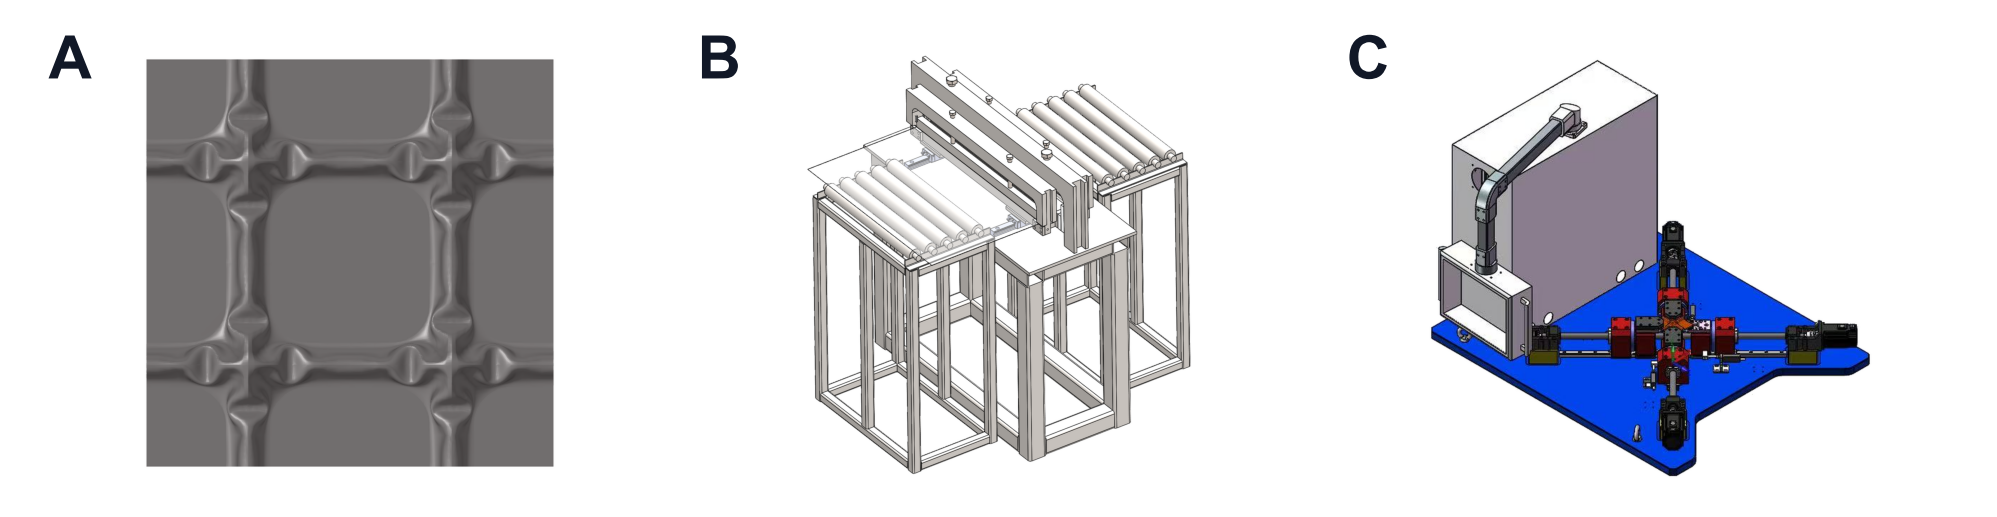
\includegraphics[width=\linewidth]{assets/fig02_uploaded_model_process_overview.png}
\end{center}
\smallnote{Selected profile $\rightarrow$ patented processing machine $\rightarrow$ four-axis specimen platform. The process figure is used as design and preparation context, not as a dimensional CAD claim.}

\vspace{0.7ex}
\begin{center}
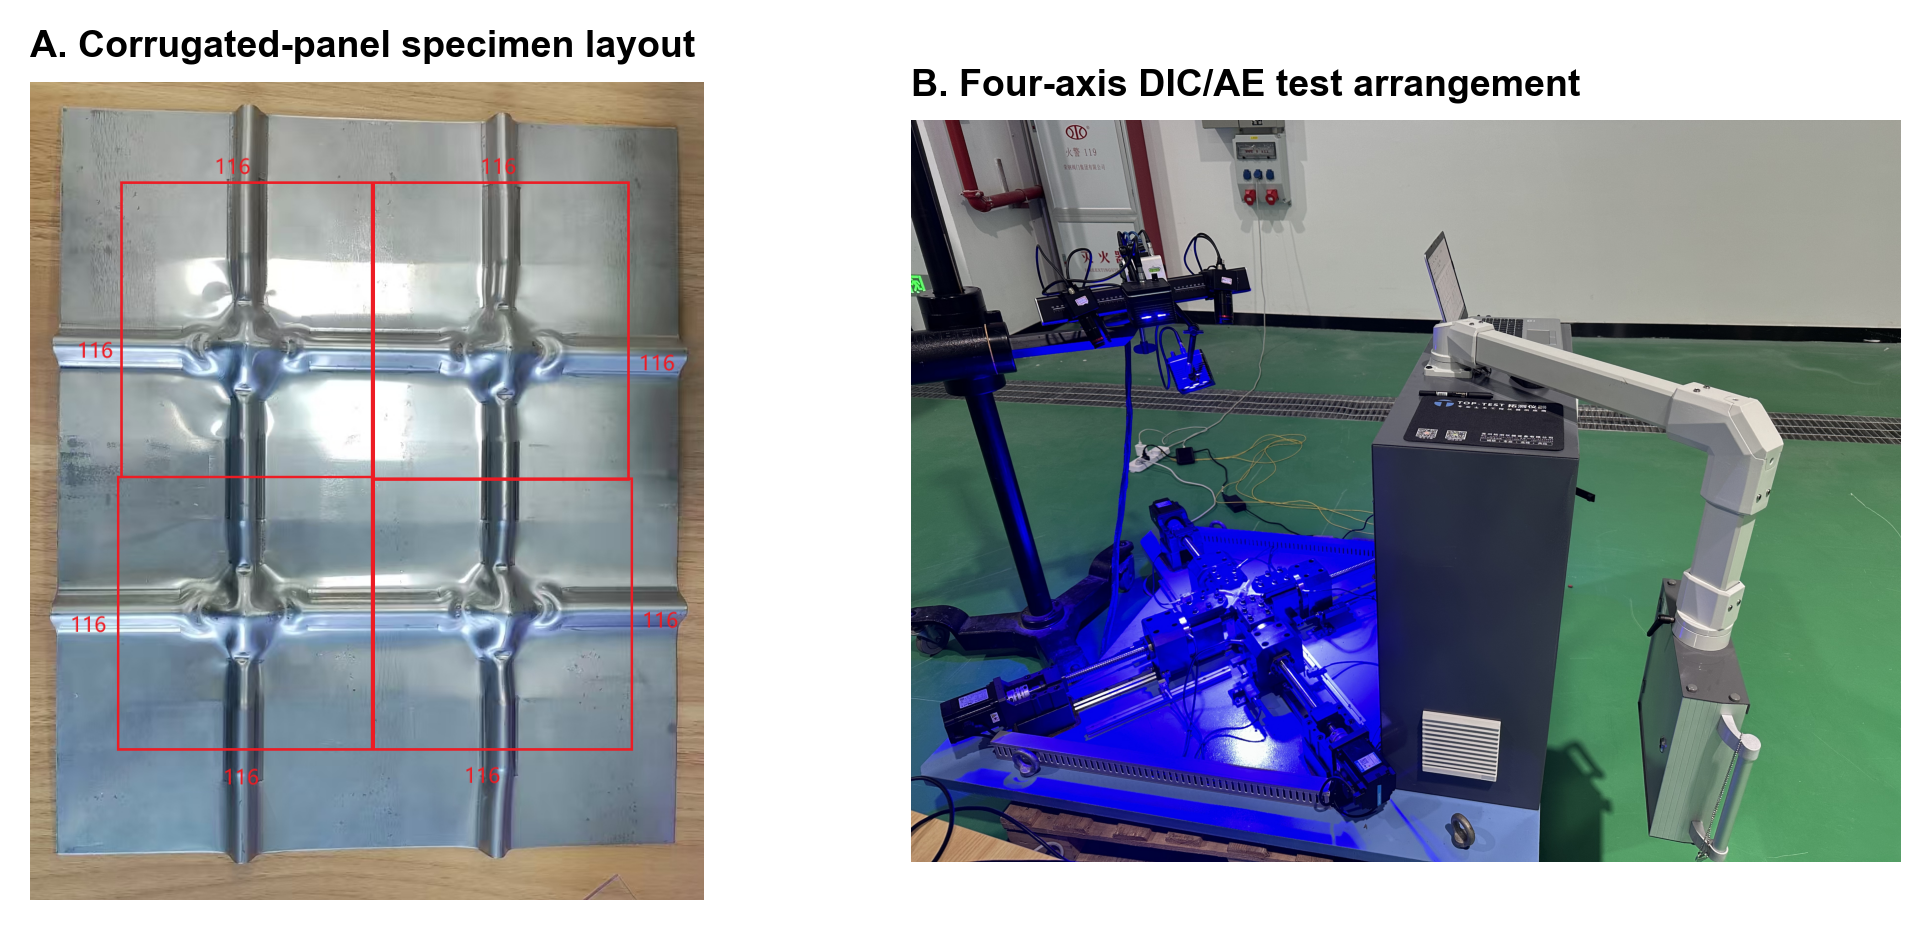
\includegraphics[width=\linewidth,height=18.0cm,keepaspectratio]{assets/fig02_experimental_setup_context.png}
\end{center}
\smallnote{Specimen extraction, DIC field of view, and mechanical setup connect the formed profile to the DIC/AE tests.}

\vspace{0.5ex}
\compacttable
\renewcommand{\arraystretch}{1.12}
\begin{tabular}{@{}>{\bfseries}p{0.20\linewidth}p{0.33\linewidth}p{0.35\linewidth}@{}}
\toprule
Experiment & Direct question & Measured output \\
\midrule
DIC/PLC & How does corrugation release imposed strain? & synchronized strain span, geometry-fixed ROI hierarchy \\
AE & When does cyclic activity concentrate? & relabeled cycle windows and damage-evolution screen \\
LN$_2$ assembly & Does pressure-retention testing verify assembly integrity after thermal cycling? & pressure-hold and helium leak checks across five LN$_2$ cycles \\
\bottomrule
\end{tabular}

\[
\bar{u}_k=\frac{1}{4}\sum_{a=1}^{4}u_{a,k},
\qquad
S_i=\frac{dP_{95}(|\varepsilon_x|)_i}{d\bar{u}},
\qquad
\Psi_i=A_iq_i^2
\]
\smallnote{The evidence chain is deliberately ordered: profile and processing first, DIC mechanism second, AE damage-evolution screening third, and pressure-retention testing for assembly integrity last.}
\end{posterblock}

\begin{posterblock}{white}{smucyan}{smunavy}{smuice}{R1. Results: DIC/PLC Mechanism Evidence}
\centering
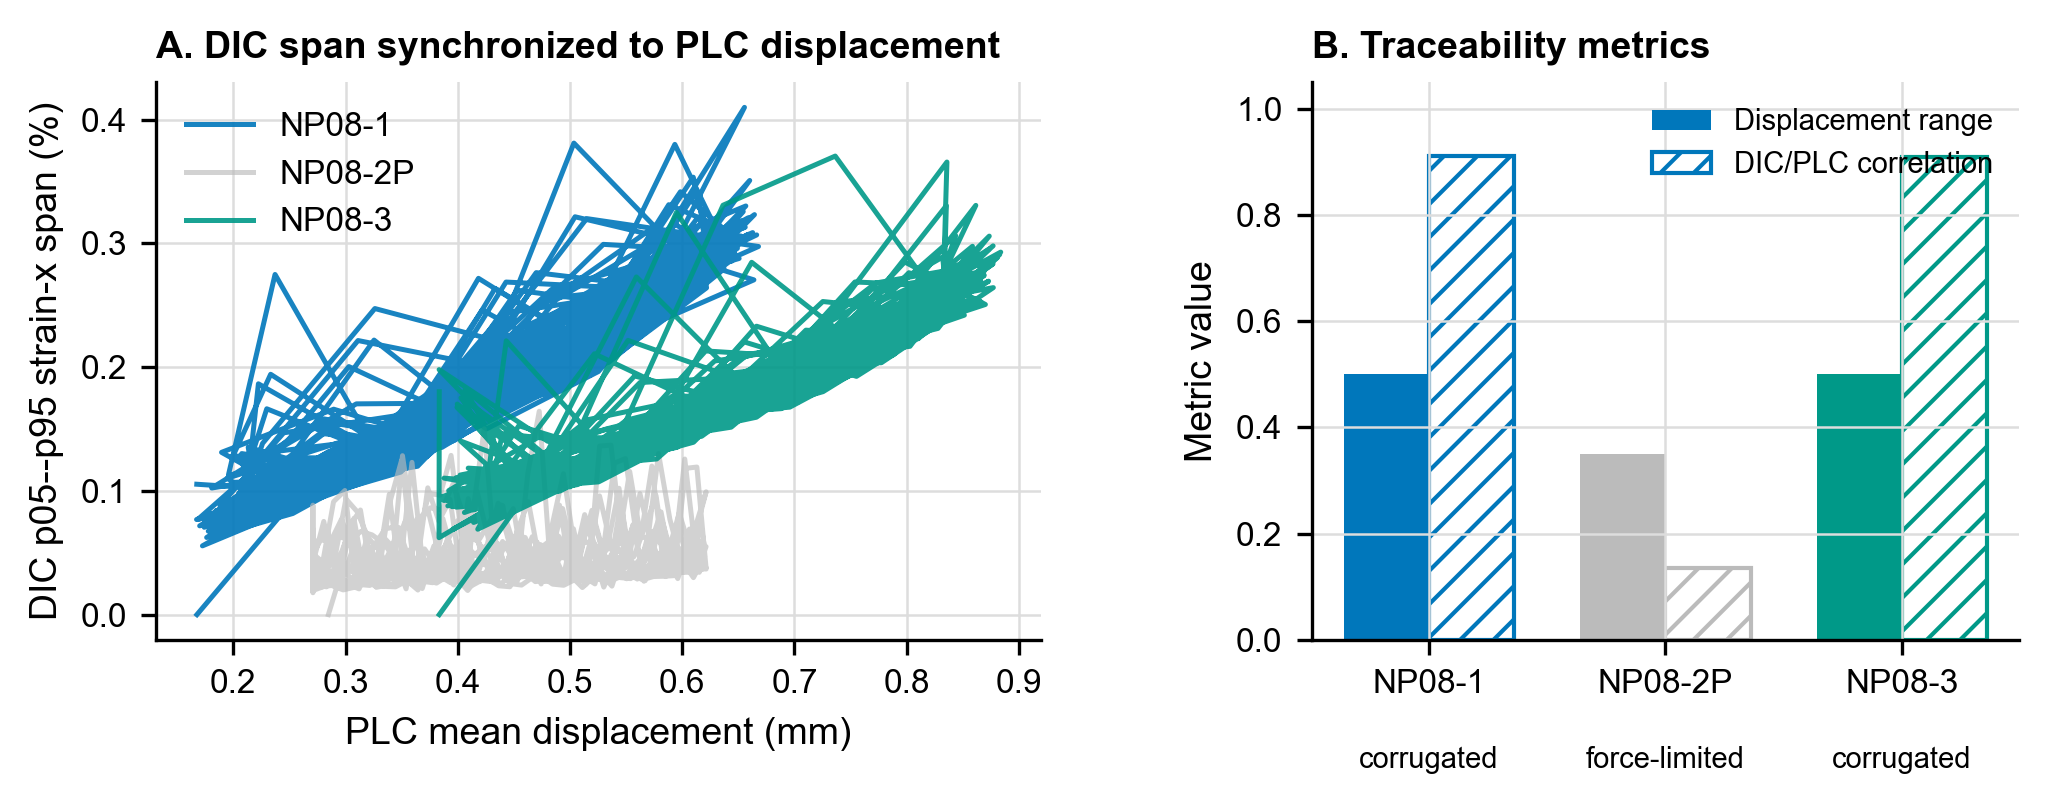
\includegraphics[width=\linewidth,height=15.8cm,keepaspectratio]{assets/fig02_dic_plc_traceability.png}
\smallnote{DIC strain span follows imposed PLC mean displacement.}

\vspace{0.6ex}
\centering
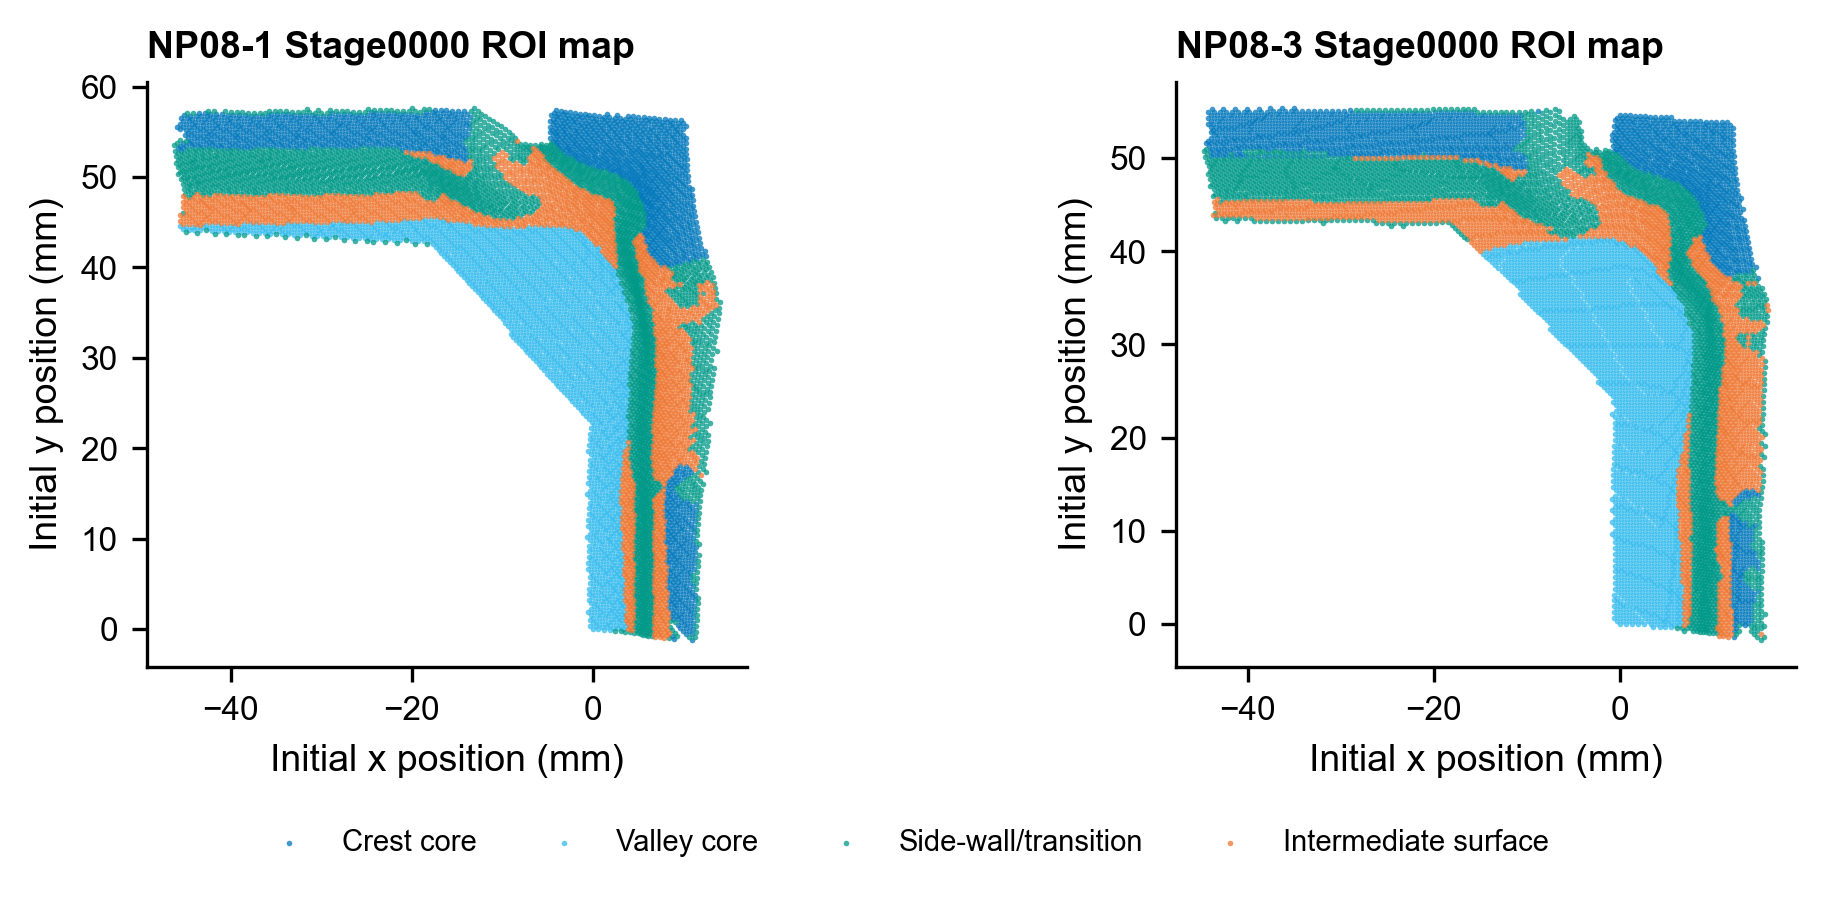
\includegraphics[width=\linewidth,height=18.2cm,keepaspectratio]{assets/fig03_dic_geometry_roi_map.png}
\smallnote{Initial geometry defines persistent ROI labels.}

\vspace{0.6ex}
\centering
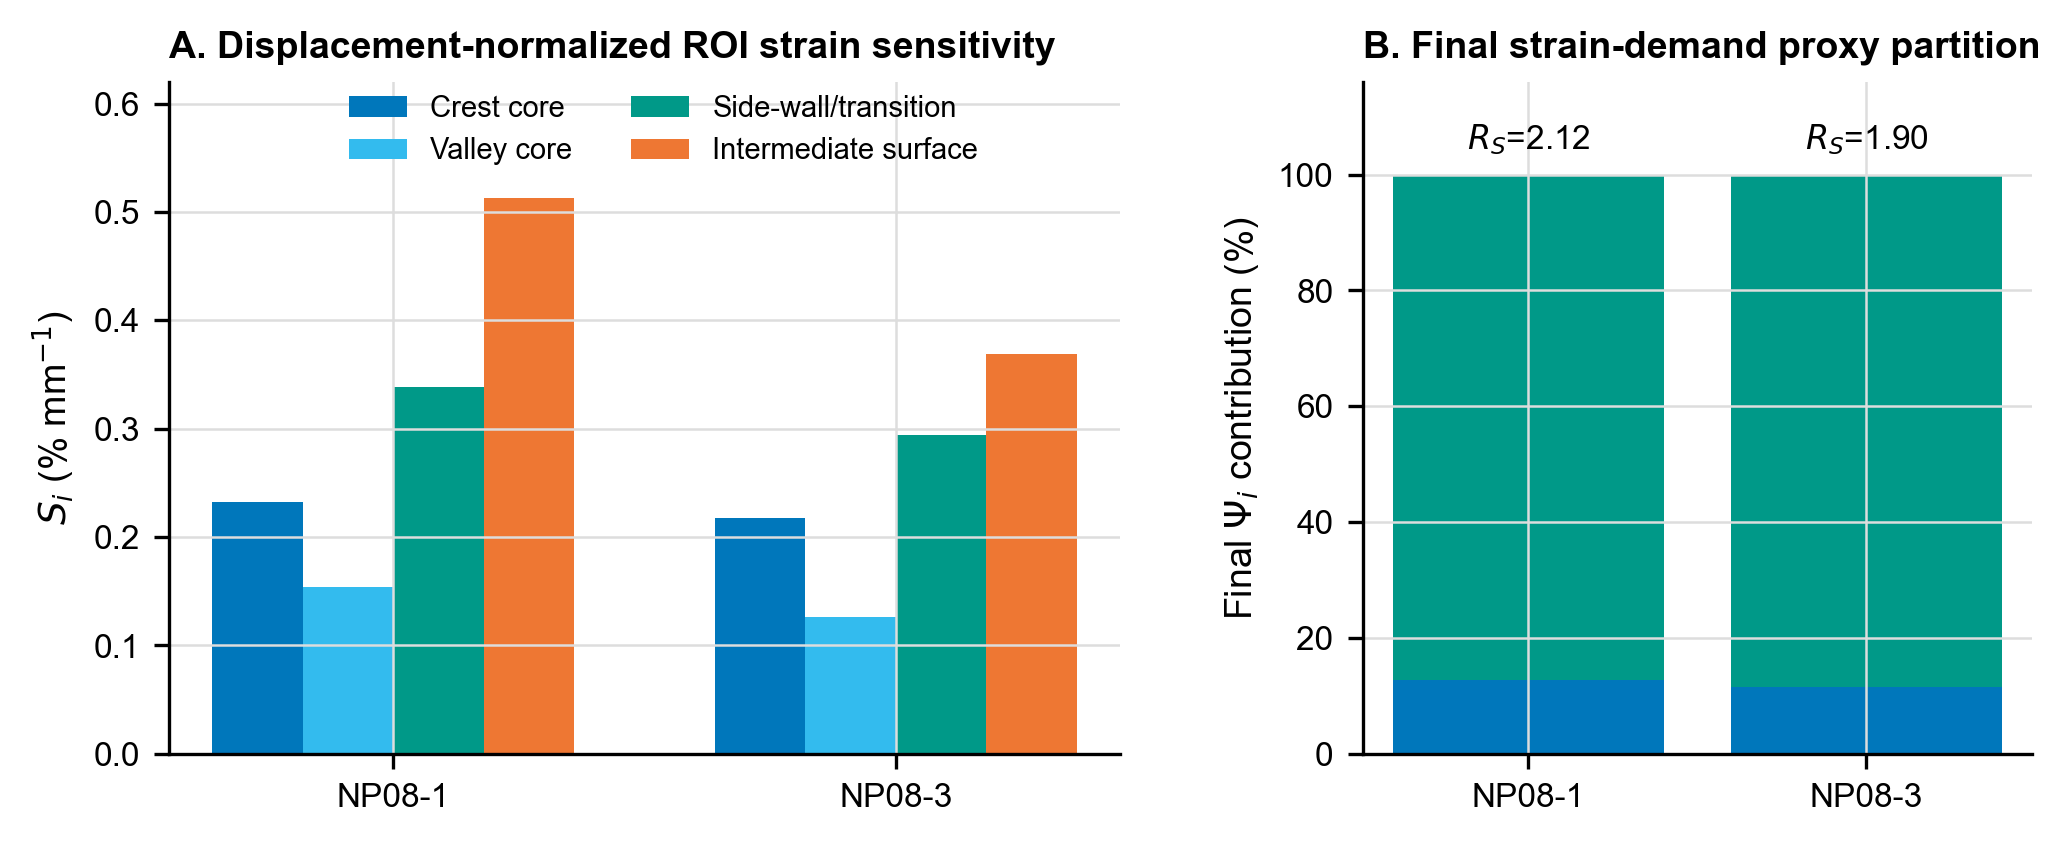
\includegraphics[width=\linewidth,height=14.8cm,keepaspectratio]{assets/fig03_dic_roi_partition.png}
\smallnote{High-deformation ROIs carry most final strain demand.}

\vspace{0.5ex}
\compacttable
\renewcommand{\arraystretch}{1.12}
\begin{tabular}{@{}>{\bfseries}p{0.32\linewidth}>{\centering\arraybackslash}p{0.18\linewidth}>{\centering\arraybackslash}p{0.18\linewidth}p{0.22\linewidth}@{}}
\toprule
Metric & NP08-1 & NP08-3 & Interpretation \\
\midrule
Sensitivity ratio $R_S$ & 2.117 & 1.896 & high-ROI response is about 2x core response \\
High-deformation area & 54.28\% & 53.96\% & deformation path occupies about half the map \\
Final strain-demand share & 87.2\% & 88.4\% & most demand stays in compliant regions \\
\bottomrule
\end{tabular}

\vspace{0.6ex}
\textbf{Mechanism result.} Corrugated specimens show repeated ROI hierarchy: side-wall/transition and intermediate surfaces absorb the imposed displacement while crest/valley cores remain lower-demand regions.
\end{posterblock}

\end{column}

\separatorcolumn

\begin{column}{\colwidth}

\begin{posterblock}{white}{smured}{smugold}{smucream!70}{R2. Results: AE Activity and Assembly Integrity Checks}
\begin{columns}[t,totalwidth=\linewidth]
\begin{column}{0.34\linewidth}
\centering
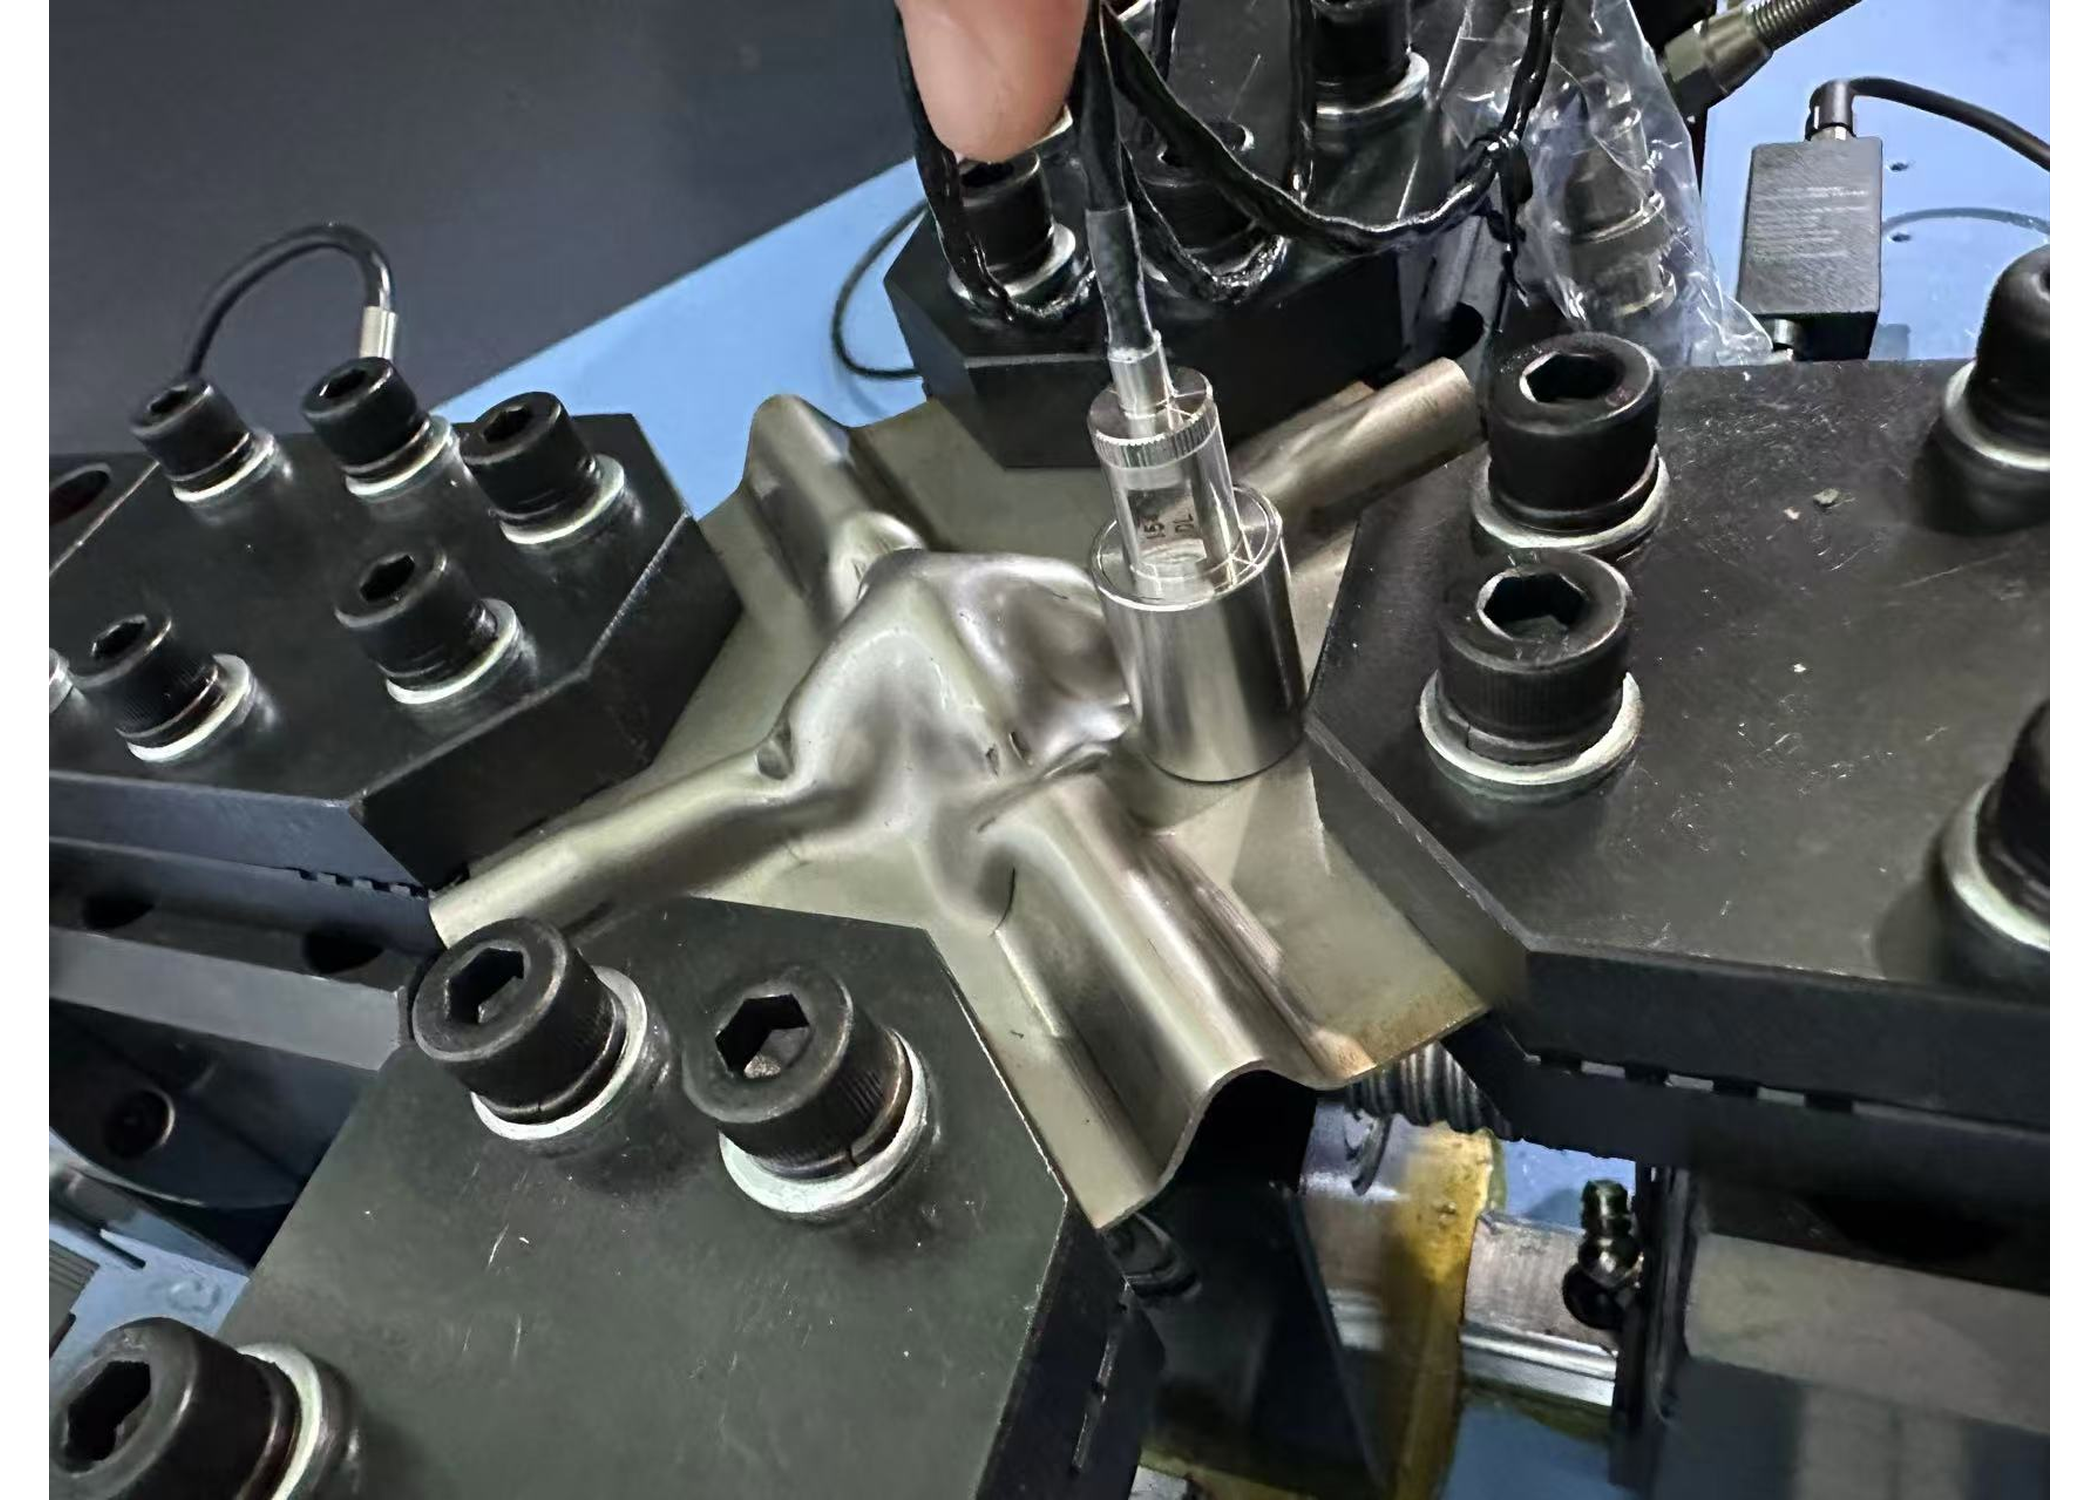
\includegraphics[width=\linewidth]{assets/fig04a_uploaded_ae_sensor_installation_photo.png}
\smallnote{AE sensors were mounted during the same four-axis loading context.}
\end{column}
\hfill
\begin{column}{0.62\linewidth}
\compacttable
\renewcommand{\arraystretch}{1.12}
\begin{tabular}{@{}>{\bfseries}p{0.25\linewidth}p{0.60\linewidth}@{}}
\toprule
Rule & Interpretive use \\
\midrule
Relabel cycles & PLC peak counting resets the AE coordinate before interpretation. \\
Track features & amplitude, high-amplitude fraction, and energy indicate cyclic activity. \\
Keep boundary & feature trends screen damage evolution; they do not alone prove cracks. \\
\bottomrule
\end{tabular}
\end{column}
\end{columns}

\centering
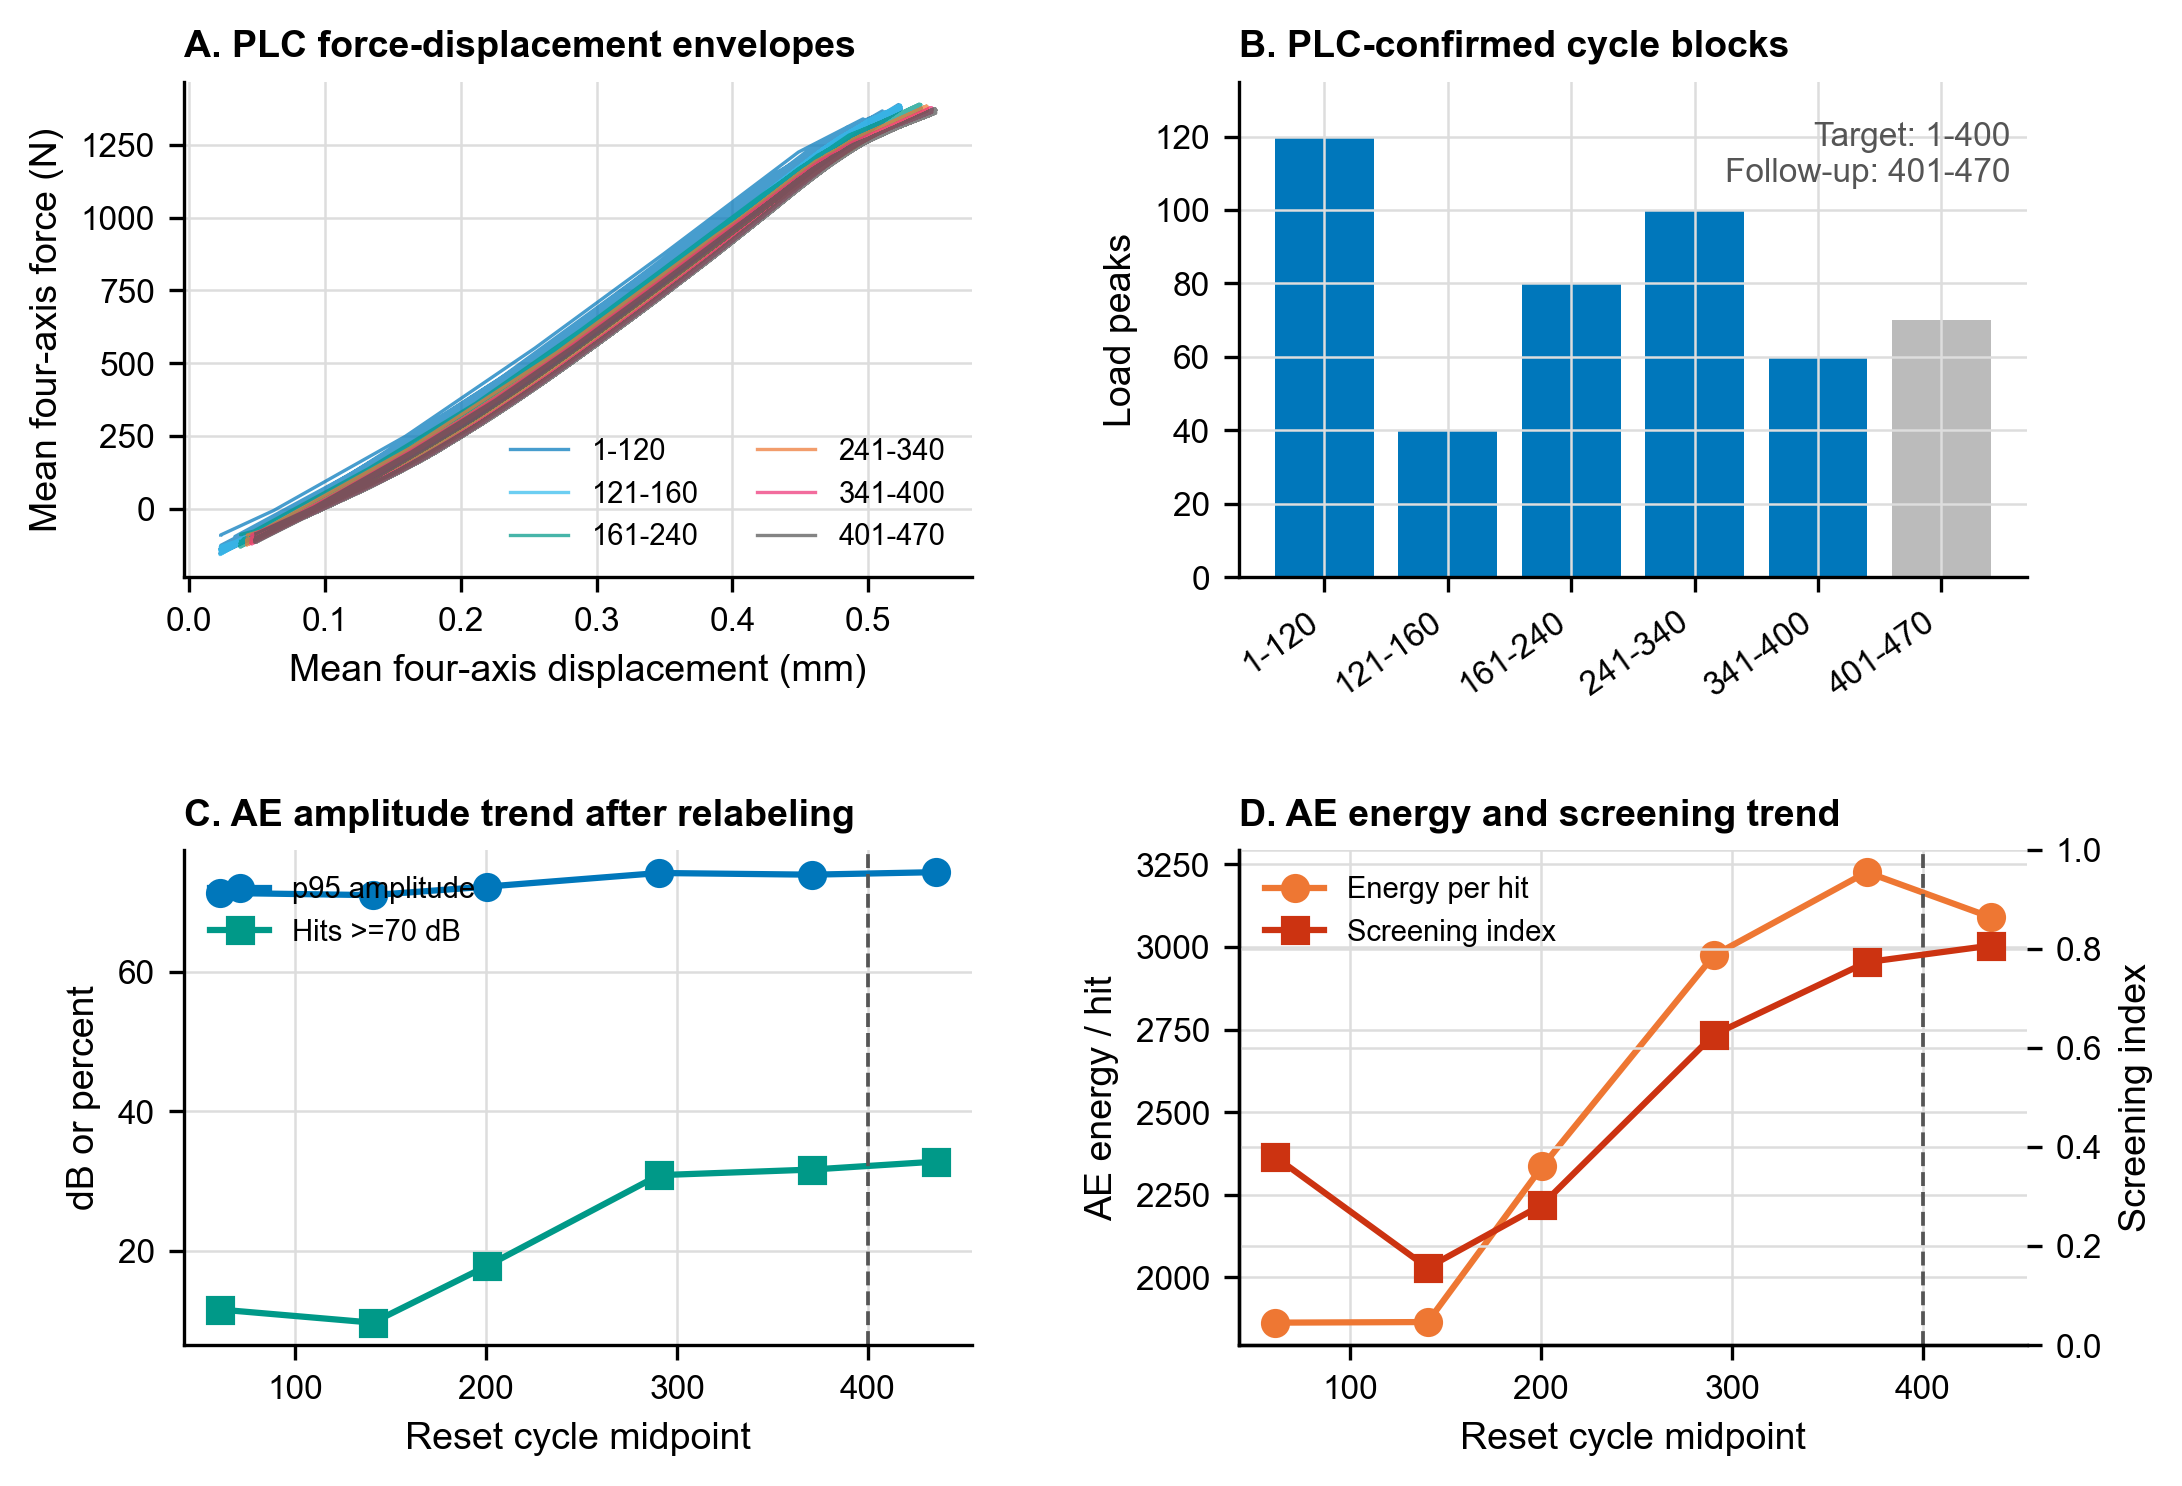
\includegraphics[width=\linewidth]{assets/fig04b_ae_cyclic_force_alignment.png}
\smallnote{PLC peak counting defines reset cycles 1--400 and follow-up 401--470.}

\vspace{0.65ex}
\centering
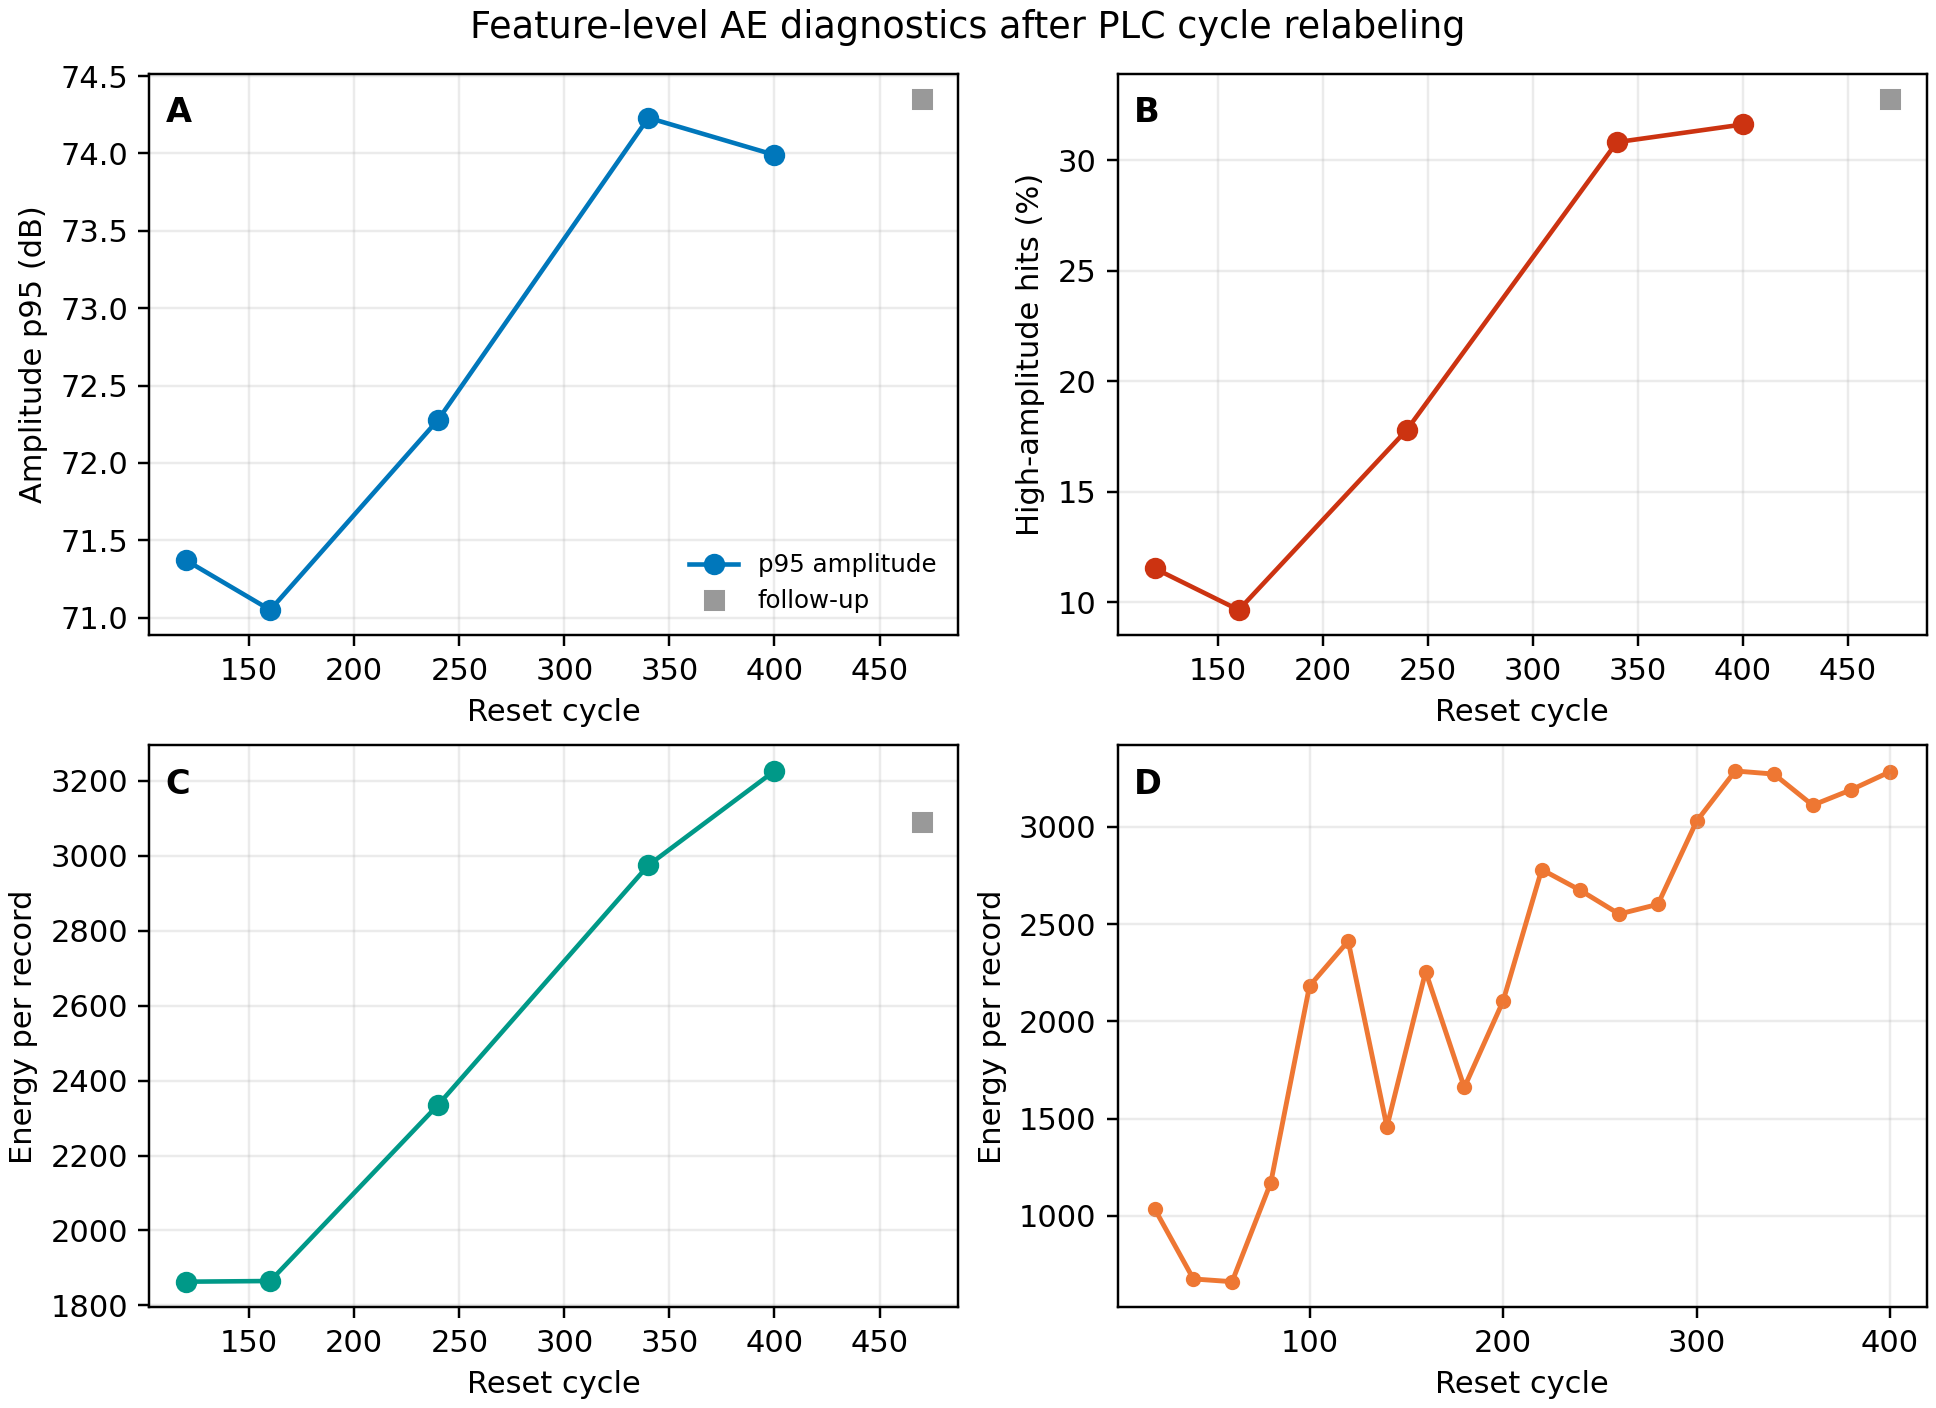
\includegraphics[width=\linewidth]{assets/fig04c_ae_full_feature_diagnostics.png}
\smallnote{Damage-evolution screen: p95 amplitude, high-amplitude fraction, and energy increase toward the late reset-cycle window.}

\vspace{0.65ex}
\centering
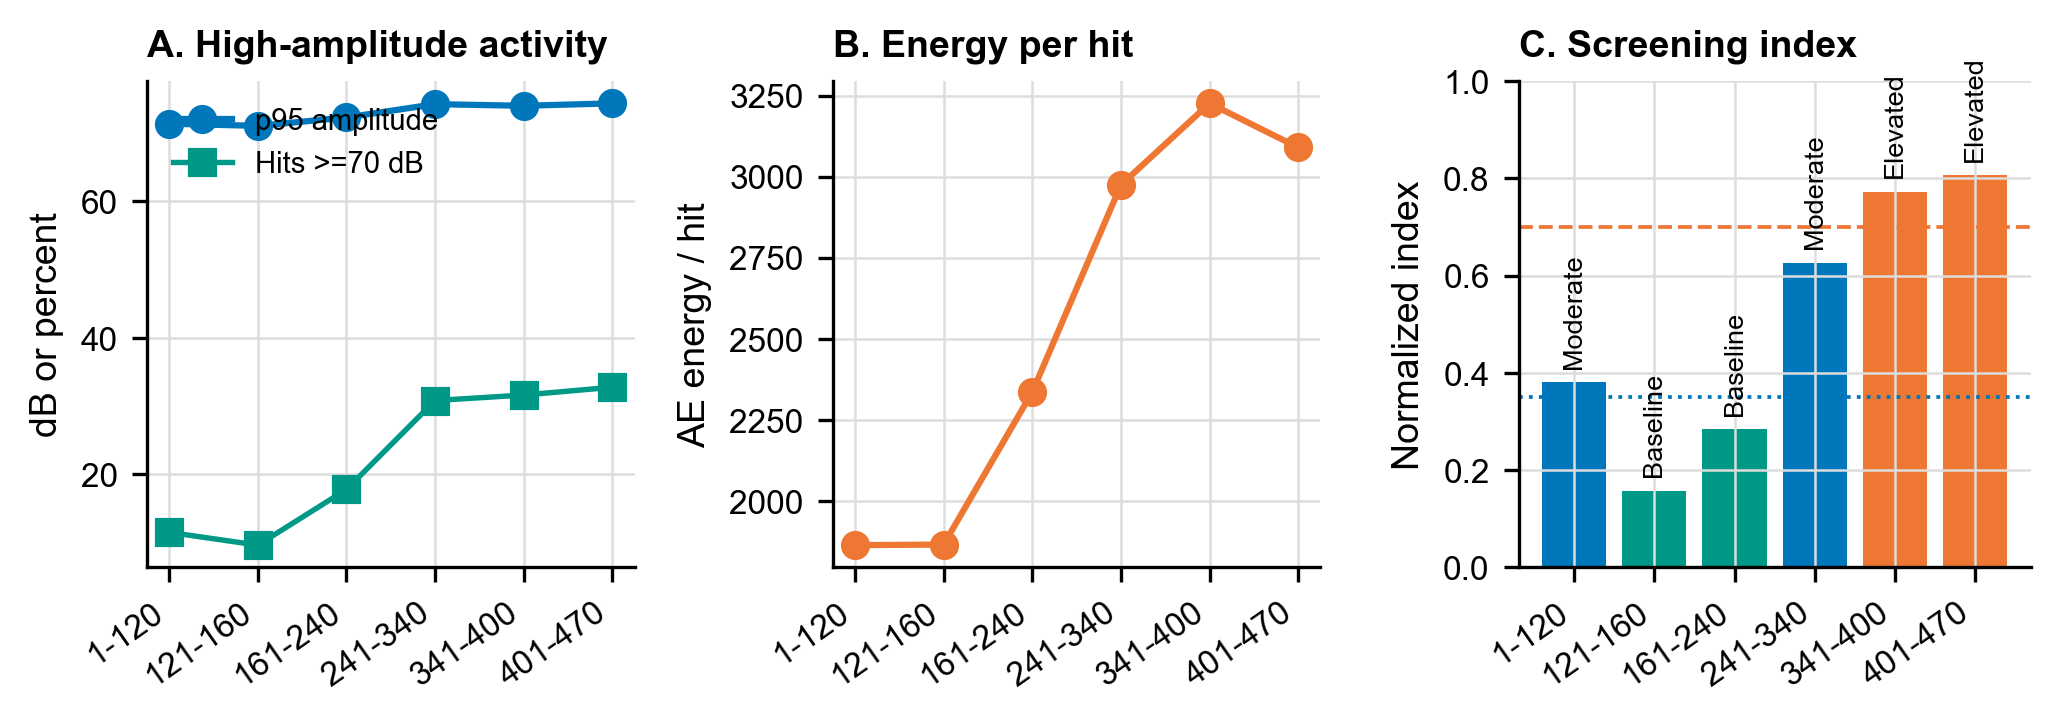
\includegraphics[width=\linewidth]{assets/fig04_ae_feature_monitoring.png}
\smallnote{Screening index ranks cycles 341--400 as the inspection-priority window.}

\vspace{0.6ex}
\metric{31.63\%}{records above 70 dB}
\hfill
\metric{$3.23\times10^3$}{energy per hit}
\hfill
\metric{125 kHz}{median frequency}
\hfill
\metric{1.17M}{feature records}

\vspace{0.7ex}
\begin{center}
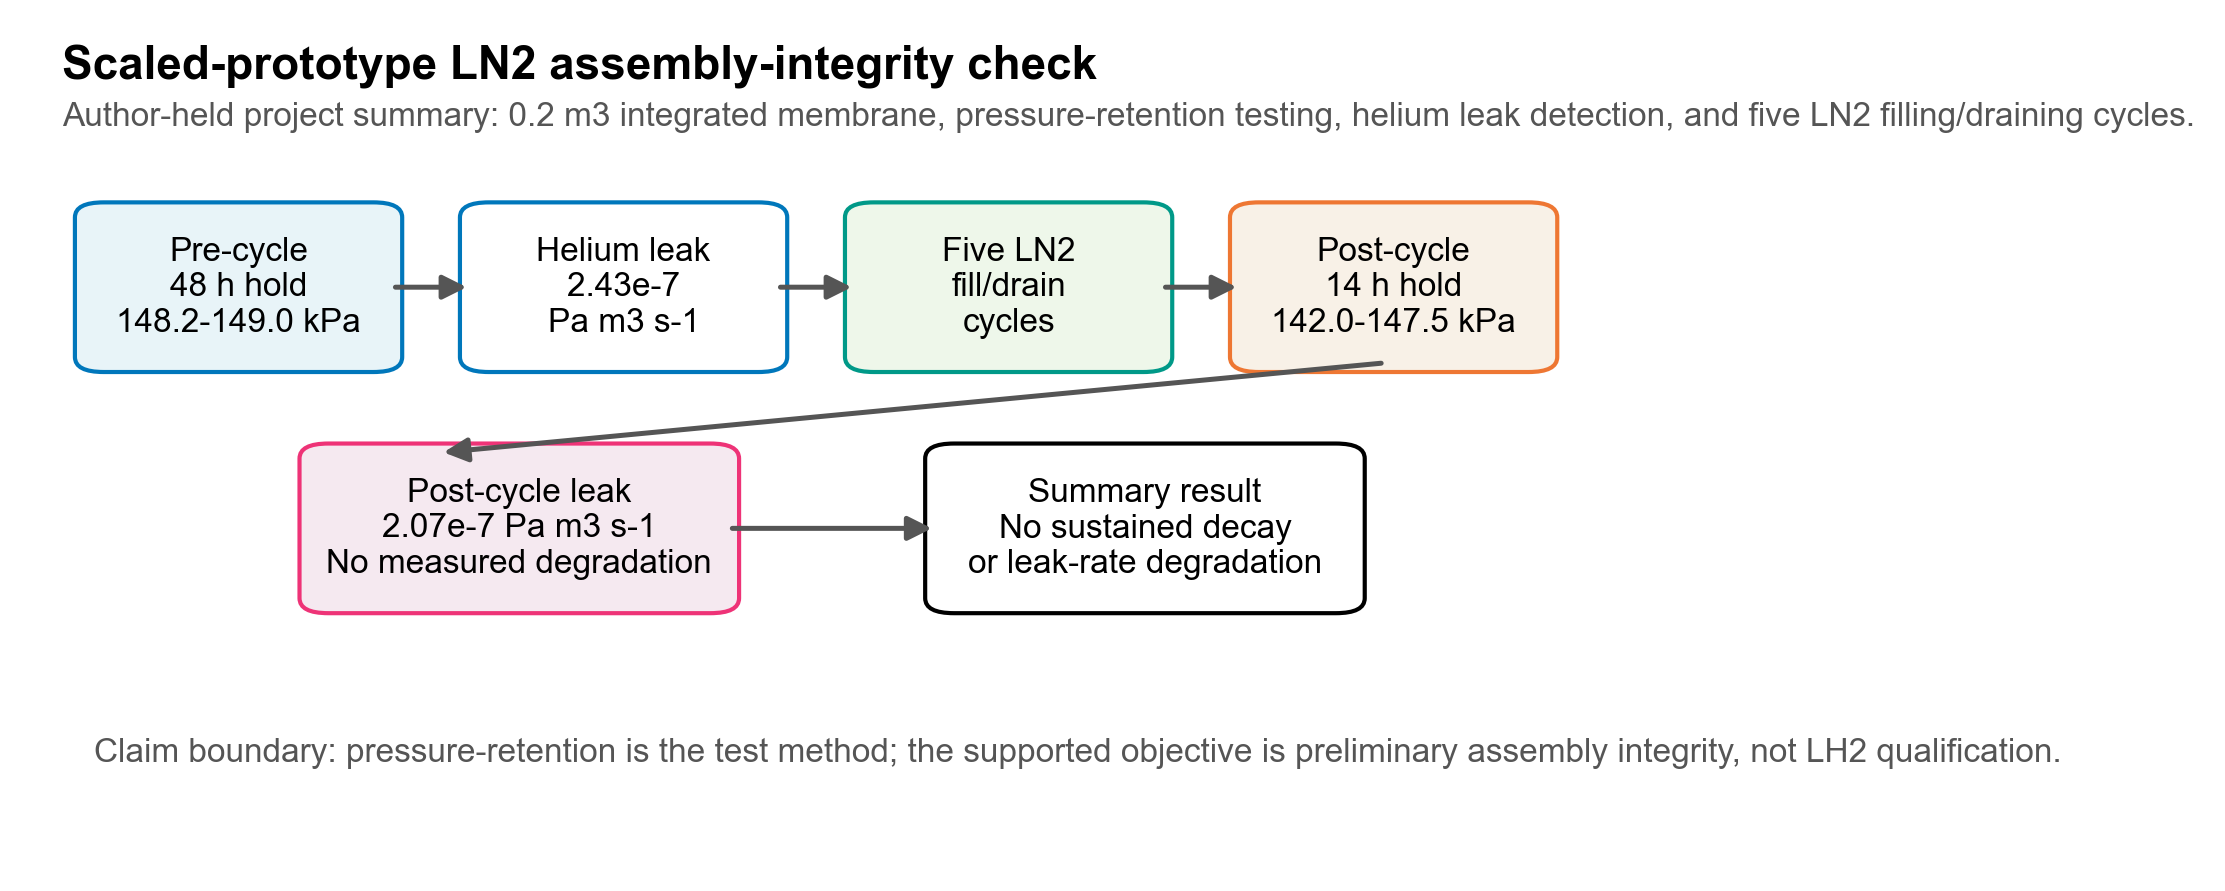
\includegraphics[width=\linewidth,height=17.2cm,keepaspectratio]{assets/fig05_ln2_integrity_gate.png}
\end{center}
\smallnote{Pressure-hold and helium leak-rate checks are the test method; the objective is to verify assembled-membrane integrity before and after five LN$_2$ filling/draining cycles.}

\compacttable
\renewcommand{\arraystretch}{1.10}
\begin{tabular}{@{}>{\bfseries}p{0.36\linewidth}p{0.52\linewidth}@{}}
\toprule
Check & Result \\
\midrule
Pre-cycle hold & 48 h at 148.2--149.0 kPa abs. \\
Post-cycle hold & 14 h at 142.0--147.5 kPa abs. \\
Pre-cycle leak & $2.43\times10^{-7}$ Pa m$^3$ s$^{-1}$ \\
Post-cycle leak & $2.07\times10^{-7}$ Pa m$^3$ s$^{-1}$ \\
\bottomrule
\end{tabular}
\end{posterblock}

\begin{posterblock}{white}{smublue}{smucyan}{smulight}{D. Discussion: What the Evidence Supports}
\compacttable
\renewcommand{\arraystretch}{1.14}
\begin{tabular}{@{}>{\bfseries}p{0.20\linewidth}p{0.29\linewidth}p{0.30\linewidth}p{0.13\linewidth}@{}}
\toprule
Layer & Supports & Does not claim & Evidence panel \\
\midrule
DIC/PLC & corrugation-driven strain redistribution & service lifetime & R1 \\
AE & late-cycle inspection-priority window & crack growth proof & R2-AE \\
LN$_2$ & preliminary assembly integrity & LH$_2$ qualification & R2-LN$_2$ \\
\bottomrule
\end{tabular}

\vspace{0.9ex}
\begin{itemize}\tightlist
\item The strongest evidence is mechanism evidence from synchronized DIC/PLC and ROI mapping.
\item AE is useful after relabeling because it ranks when inspection attention should focus.
\item LN$_2$ pressure-retention testing is necessary but not sufficient for final LH$_2$ service readiness.
\end{itemize}
\end{posterblock}

\begin{posterblock}{white}{smunavy}{smucyan}{smuice}{C. Conclusions and Next Gates}
\begin{columns}[t,totalwidth=\linewidth]
\begin{column}{0.48\linewidth}
\heading{Conclusions}
\begin{enumerate}\tightlist
\item Corrugation redistributes strain into traceable geometry-defined ROIs.
\item The late AE reset window gives an inspection-priority signal.
\item Pre/post LN$_2$ pressure and leak checks support preliminary assembly integrity.
\end{enumerate}
\end{column}
\hfill
\begin{column}{0.48\linewidth}
\heading{Next gates}
\begin{enumerate}\tightlist
\item Repeat coupon tests with ROI uncertainty.
\item Add cryogenic DIC and waveform-level AE.
\item Report full acceptance pressure/leak records under LH$_2$-relevant criteria.
\end{enumerate}
\end{column}
\end{columns}

\vspace{0.8ex}
\compacttable
\renewcommand{\arraystretch}{1.08}
\begin{tabular}{@{}>{\bfseries}p{0.25\linewidth}p{0.65\linewidth}@{}}
\toprule
ICEC/ICMC record & P1-061, Poster Session I, Exhibition Hall (111+112), June 23, 2026, 14:00--16:00 \\
Claim boundary & The evidence supports staged validation under the tested conditions; completed LH$_2$ service qualification remains outside the present scope. \\
\bottomrule
\end{tabular}
\end{posterblock}

\end{column}

\separatorcolumn
\end{columns}

\end{frame}
\end{document}
